\subsubsection{Calculation Method}

The safety score is a composite metric designed to evaluate the environmental safety conditions for each weather station across Austria. It combines the following variables:

\begin{itemize}
    \item \textbf{Average Sunshine Hours}: Higher values are considered favorable.
    \item \textbf{Frequency of Wind Gusts}: Higher values are penalized due to increased hazard potential.
    \item \textbf{Frequency of Frost Days}: Higher values indicate harsher conditions and are penalized.
    \item \textbf{Frequency of Heat Days}: Moderately penalized to reflect discomfort and potential risk.
\end{itemize}

The score is calculated as a weighted sum:

\begin{equation}
\text{Score} = \text{Sunshine} - 2 \cdot \text{Wind Gust Freq} - 2 \cdot \text{Frost Freq} - 1.5 \cdot \text{Heat Freq}
\end{equation}

A higher safety score indicates more favorable and stable environmental conditions.

\subsubsection{Top Station Scores}

Table~\ref{tab:top_scores} shows the top 10 station-season combinations with the highest safety scores. These stations are located exclusively in high alpine zones (\textgreater 2000\,m) within Salzburg and exhibit high sunshine hours, but still significant wind and frost frequencies.

\begin{table}[H]
\centering
\begin{tabular}{|c|c|c|c|c|}
\hline
\textbf{Season} & \textbf{Station} & \textbf{Region} & \textbf{Sunshine [h]} & \textbf{Score} \\
\hline
Spring & 15410 & Salzburg & 461.3 & 398.8 \\
Spring & 213   & Salzburg & 440.8 & 378.2 \\
Spring & 15411 & Salzburg & 394.1 & 331.2 \\
Summer & 15410 & Salzburg & 336.1 & 291.5 \\
Spring & 15322 & Salzburg & 340.9 & 283.9 \\
Summer & 213   & Salzburg & 319.8 & 278.3 \\
Summer & 15411 & Salzburg & 279.7 & 243.9 \\
Winter & 15410 & Salzburg & 303.8 & 239.3 \\
Winter & 213   & Salzburg & 296.1 & 232.3 \\
Winter & 15411 & Salzburg & 294.0 & 231.4 \\
\hline
\end{tabular}
\caption{Top 10 Safety Scores by Station and Season}
\label{tab:top_scores}
\end{table}

\subsubsection{Visual Interpretation}

\begin{figure}[H]
    \centering
    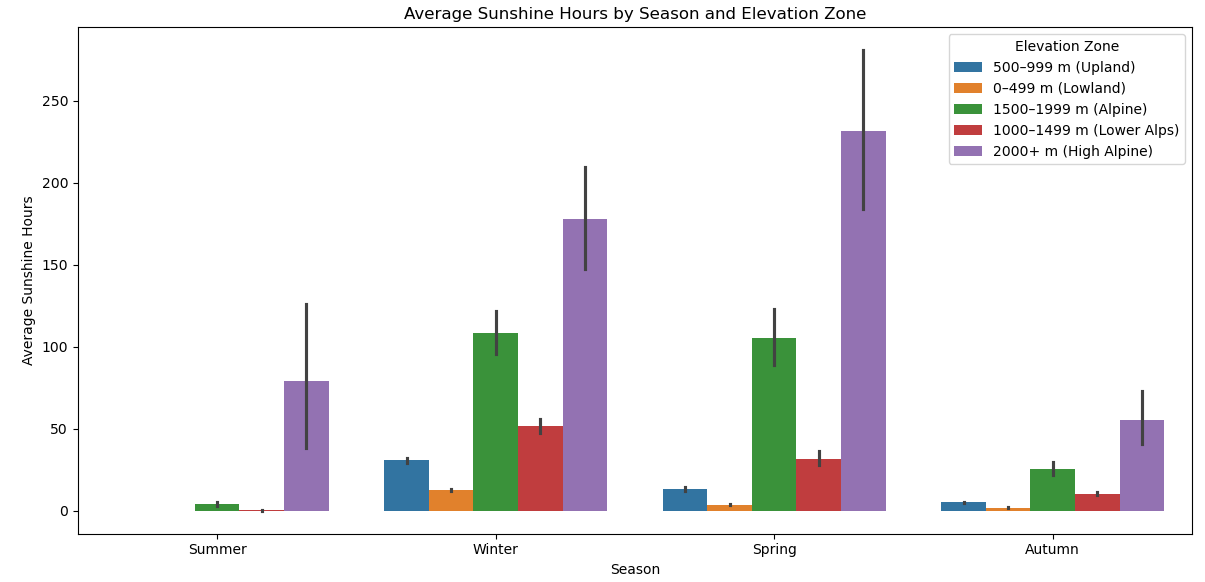
\includegraphics[width=0.45\textwidth]{img/sunshine_by_season_zone.png}
    \caption{Average Sunshine Hours by Season and Elevation Zone}
    \label{fig:sunshine}
\end{figure}

Figure~\ref{fig:sunshine} shows that the high alpine zone consistently records higher average sunshine hours across all seasons, especially in spring. This contributes positively to their safety scores.

\begin{figure}[H]
    \centering
    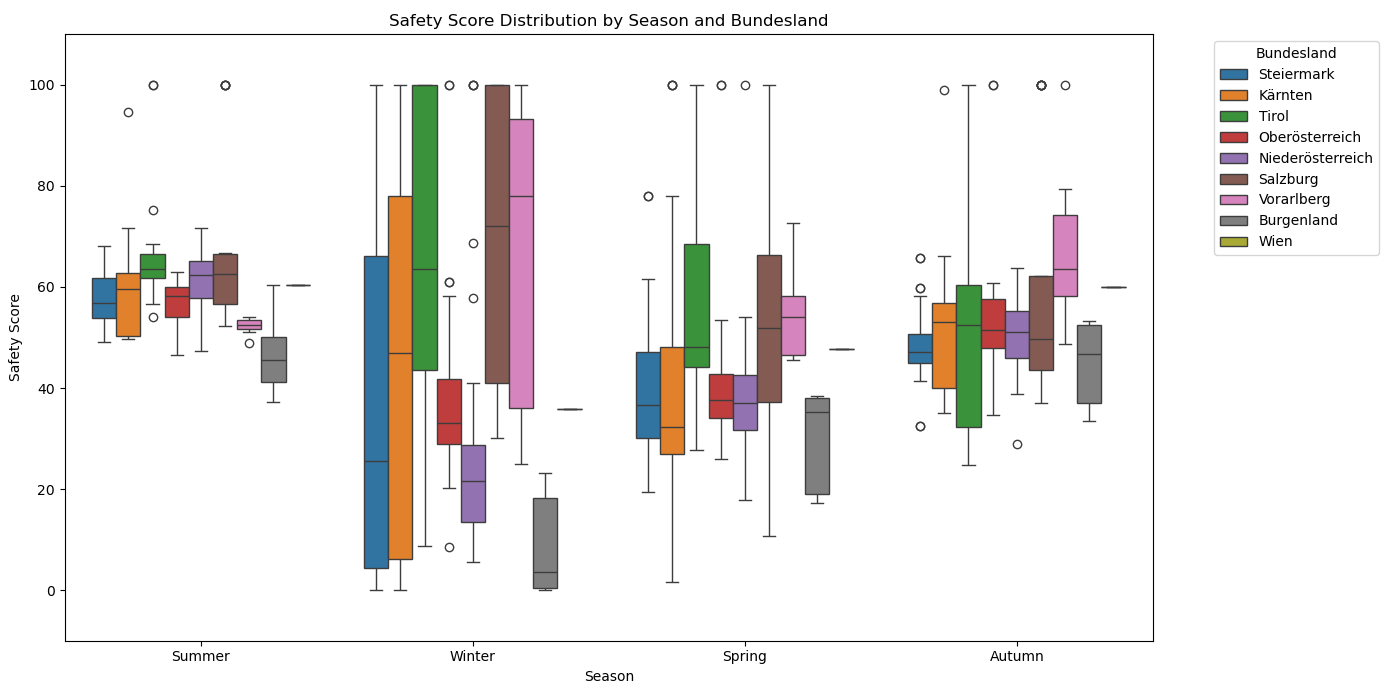
\includegraphics[width=0.45\textwidth]{img/safety_score_boxplot.png}
    \caption{Safety Score Distribution by Season and Bundesland}
    \label{fig:safety_boxplot}
\end{figure}

Figure~\ref{fig:safety_boxplot} presents the distribution of safety scores. Salzburg, Tirol, and Vorarlberg show the highest spread and highest values in winter and spring, corresponding to high-elevation stations.

\begin{figure}[H]
    \centering
    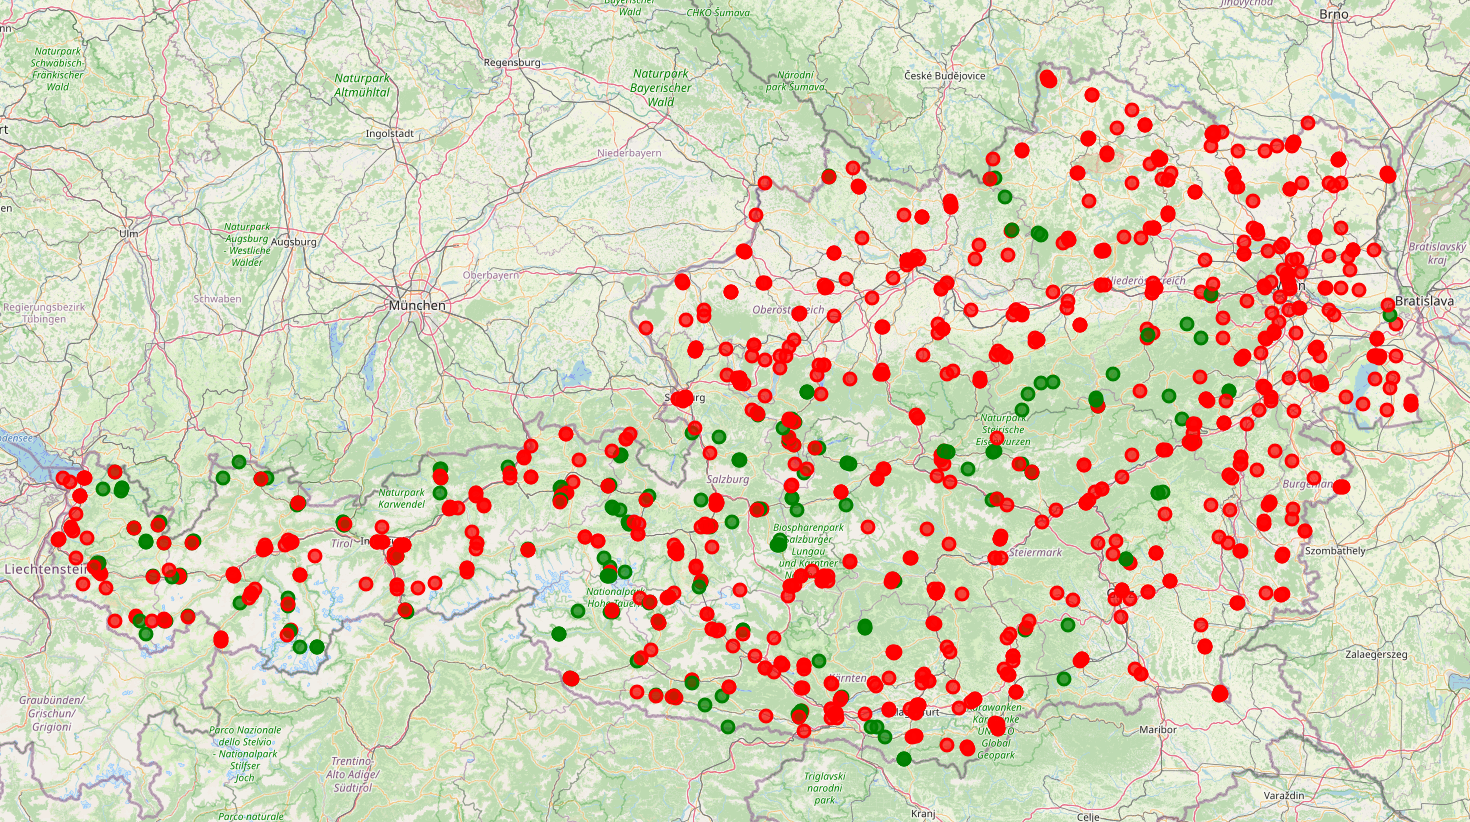
\includegraphics[width=0.45\textwidth]{img/station_map.png}
    \caption{Map of Stations by Safety Score (Green: High, Red: Low)}
    \label{fig:station_map}
\end{figure}

Figure~\ref{fig:station_map} visualizes the spatial distribution of safety scores. Green points indicate stations with relatively high safety scores, found predominantly in the Alpine regions. Red points represent stations with lower scores, more frequent in lower elevation areas.
